% !TeX root = ../defense.tex

\section{Simulations}
\frame{\sectionpage}

\begin{frame}{Spectral energy density}
\begin{equation*}
	\uncover<+->{
		\Omega_{SGWB} = \Omega_{SGWB} (f, \{\Theta_{\text{source}}, \Theta_{\text{astrophysics}}, \Theta_{\text{cosmology}}, \dots\})
	}
\end{equation*}
~\\
\uncover<+->{Depends on:}
\begin{itemize}[<+->]
	\item Source type, Mass scales, ...
	\item Location of sources, Dynamical enviornments, ...
	\item Cosmology model parameters, Mass function, ...
	\item Other observational or Intermediary effects\\~\\
\end{itemize}
\uncover<+->{Ways to calculate $\Omega_{gw}$:}
\begin{enumerate}[<+->]
	\item \textbf{Analytical approach}: For relatively simple models (e.g. inflationary gravitational waves in $\Lambda CDM$ \textcolor{gray}{\fontsize{7.5}{10}\selectfont [\href{https://www.elsevier.com/books/modern-cosmology/dodelson/978-0-12-815948-4}{Dodelson, Schmidt}]})
	
	\item \textbf{Simulation}: For Complicated models with high accuracy (e.g. \textcolor{gray}{\fontsize{7.5}{10}\selectfont [\href{https://www.sciencedirect.com/science/article/pii/S2212686416300553}{Clesse, et al.}], [\href{https://journals.aps.org/prd/abstract/10.1103/PhysRevD.98.063501}{Jenkins, et al.}]})
	
	\item \textbf{Semi-analytocal approach}: For quickly testing various complicated models whithout using too much computational resource (e.g. 
	\textcolor{gray}{\fontsize{7.5}{10}\selectfont [\href{https://iopscience.iop.org/article/10.1088/1475-7516/2021/12/012/meta}{Braglia, et al.}], [\href{https://iopscience.iop.org/article/10.1088/1742-6596/222/1/012021/meta}{Durrer}],
	[\href{https://academic.oup.com/mnras/article-abstract/506/3/3977/6317617}{Mukherjee, et al.}]
	})
\end{enumerate}
\end{frame}

\begin{frame}{Semi-Analytical approach}
\uncover<+->{$\Omega_{SGWB}(f, \{\Theta\}_{i = 0}^n) =$}
$$\uncover<+->{\frac{f}{\rho_c c^2} \int \der^n \Theta_i \int \der z} \uncover<+->{\overbrace{\frac{\der t_r}{\der z}}^{\mathrm{cosmology}}} \uncover<+->{\underbrace{\frac{\der^m \tau_{\text{merg}}(z, \Theta_j)}{\der \Theta_0 \der \Theta_1 \dots \der \Theta_m}}_{\mathrm{\shortstack{astrophysics\\ \&~ cosmology}}}} \uncover<+->{\overbrace{\frac{\der E_{\mathrm{GW}}(f_r, \Theta_k)}{\der f_r}}^{\mathrm{GW~source}}}$$\\~\\~\\

\uncover<+->{$f_r = (1+z) f$}
\end{frame}

\begin{frame}{Cosmology part}
	\uncover<1->{The cosmology is encoded in the Hubble parameter which appears in number of events which occur in a comoving volume between the cosmic times $t_r(z)$ and $t_r(z + \der z)$}\\~\\
	$$\uncover<2->{\frac{\mathrm{d}N}{\mathrm{d}z} = \dot{N}} \uncover<1->{\frac{\mathrm{d}t_r}{\mathrm{d}z}} \uncover<2->{= \frac{\dot{N}}{H(z) (1+z)}}$$\\~\\
	$$\uncover<3->{H^2(z) = H_0^2 \left[\Omega_\mathrm{r}(1+z)^4 + (\Omega_\mathrm{DM} + \Omega_\mathrm{b})(1+z)^3 + \Omega_\mathrm{k}(1+z)^2 + \Omega_\Lambda\right]}$$\\~\\
\end{frame}

\begin{frame}{Astrophysics/Cosmology part}
Following the pictrue in \textcolor{gray}{[M. Braglia, J. Garcia-Bellido, and S. Kuroyanagi, “Testing primordial black holes with multi-band observations of the stochastic gravitational wave background”, \href{https://iopscience.iop.org/article/10.1088/1475-7516/2021/12/012/meta}{\textit{Journal of Cosmology and Astroparticle Physics}, vol.2021, no.12, p.012, 2021.}]}\\~\\
\begin{equation*}
\begin{split}
\uncover<+->{\dot{N}}
\uncover<+->{
	=&\frac{\der^2 \tau_{\text{merg}} (z, m_1, m_2, \{\alpha_z, \alpha_c\})}{\der \log_{10} m_1 \der \log_{10} m_2} =
	} \\
\uncover<+->{&\qquad\qquad\qquad\underbrace{R_{\text{clust}} \frac{(m_1 + m_2)^{10/7}}{(m_1 m_2)^{5/7}} \frac{(1+z)^{\alpha_z}}{\left[1 + (M_{tot} / M_\star)\right]^{\alpha_c}}}_{\mathrm{PBH~clustering/binary~formation}}} \uncover<+->{\overbrace{f_{PBH}(m_1)f_{PBH}(m_2)}^{primordial/thermal~evolution}}
\end{split}
\end{equation*}
\end{frame}

\begin{frame}{Merger rate Calculation an PBH mass function}
~\\~\\
\begin{align*}
	\uncover<+->{
		&\frac{\der^2 \tau_{\text{merg}}^{\mathrm{our~model}}(z, m_1, m_2)}{\der \log_{10} m_1 \der \log_{10} m_2} = R_{\text{clust}} \frac{(m_1 + m_2)^{10/7}}{(m_1 m_2)^{5/7}} f_{PBH}(m_1)f_{PBH}(m_2)\\~\\~\\
	}
	\uncover<+->{
		\text{To fix } R_{\text{clust}}:\quad
		&\int \der m_1 \int \der m_2 \frac{\der^2 \tau_{\text{merg}}^{\mathrm{our~model}}(0, m_1, m_2)}{\der \log_{10} m_1 \der \log_{10} m_2} = 38~yr^{-1} Gpc^{-1}\\~\\~\\
	}
	\uncover<+->{
		&f_{PBH} (m, \{\boxed{\sigma_{PBH}}, \mu\}) = F_0 \frac{1}{\sqrt{2\pi} \sigma_{PBH} m} \exp\left[{-\frac{(\log_{10}\frac{m}{\mu})^2}{2 \sigma_{PBH}^2}}\right]\\~\\~\\
	}
\end{align*}
\end{frame}

\begin{frame}{Source part}
\begin{columns}
\begin{column}{0.6\linewidth}
\begin{align*}
\uncover<+->{
	&\frac{\mathrm{d}E_{\mathrm{GW}}(\Theta_i)}{\mathrm{d}f_r} = \frac{(G\pi)^{2/3}\mathcal{M}_c^{3/5}}{3} \mathcal{G}(f_r, \Theta)\\~\\
}
\uncover<+->{
	&\mathcal{M}_c = \frac{(m_1 + m_2)^{3/5}}{(m_1 + m_2)^{1/5}}\\~\\
}
\end{align*}
\begin{equation*}
\uncover<+->{
	\mathcal{G}(f_r) = 
	\begin{cases}
		\uncover<+->{
			f_r^{-1/3} \qquad & f_r < f_{\mathrm{merg}}\\
		}
		\uncover<+->{
			\frac{f_r^{2/3}}{f_{\mathrm{merg}}} \qquad & f_{\mathrm{merg}} \leq f_r < f_{\mathrm{ring}}\\
		}
		\uncover<+->{
			\frac{1}{f_{\mathrm{merg}} f_{\mathrm{ring}}^{4/3}} \left(\frac{f_r}{1 + \left(\frac{f_r - f_{\mathrm{ring}}}{f_w / 2}\right)^2}\right)^2 \qquad & f_{\mathrm{ring}} \leq f_r < f_{\mathrm{cut}}
		}
	\end{cases}
}
\end{equation*}
\end{column}


\begin{column}{0.4\linewidth}
\begin{align*}
\uncover<+->{
	f_x = &\frac{c^3}{\pi G M_{tot}} \left(a_1 \eta^2 + a_2 \eta + a_3\right)\\~\\
}
\uncover<+->{
	&M_{tot} = m_1 + m_2\\~\\
}
\uncover<+->{
	&\eta = \frac{m_1 + m_2}{M_{tot}^2}\\~\\
}
\end{align*}

\end{column}
\end{columns}
\end{frame}

\begin{frame}{From spectral energy density to wave forms}
\begin{columns}
\begin{column}{0.5\linewidth}
\begin{tikzpicture}%[node distance=1em and 2ex,font=\small]
\uncover<+->{
	\node[flowbox,fb-muted] (model) {
		\fbtitle{page 11}%\vphantom{yÖ}
		\nodepart{two}
		\begin{minipage}{0.9\linewidth}
			%\centering
			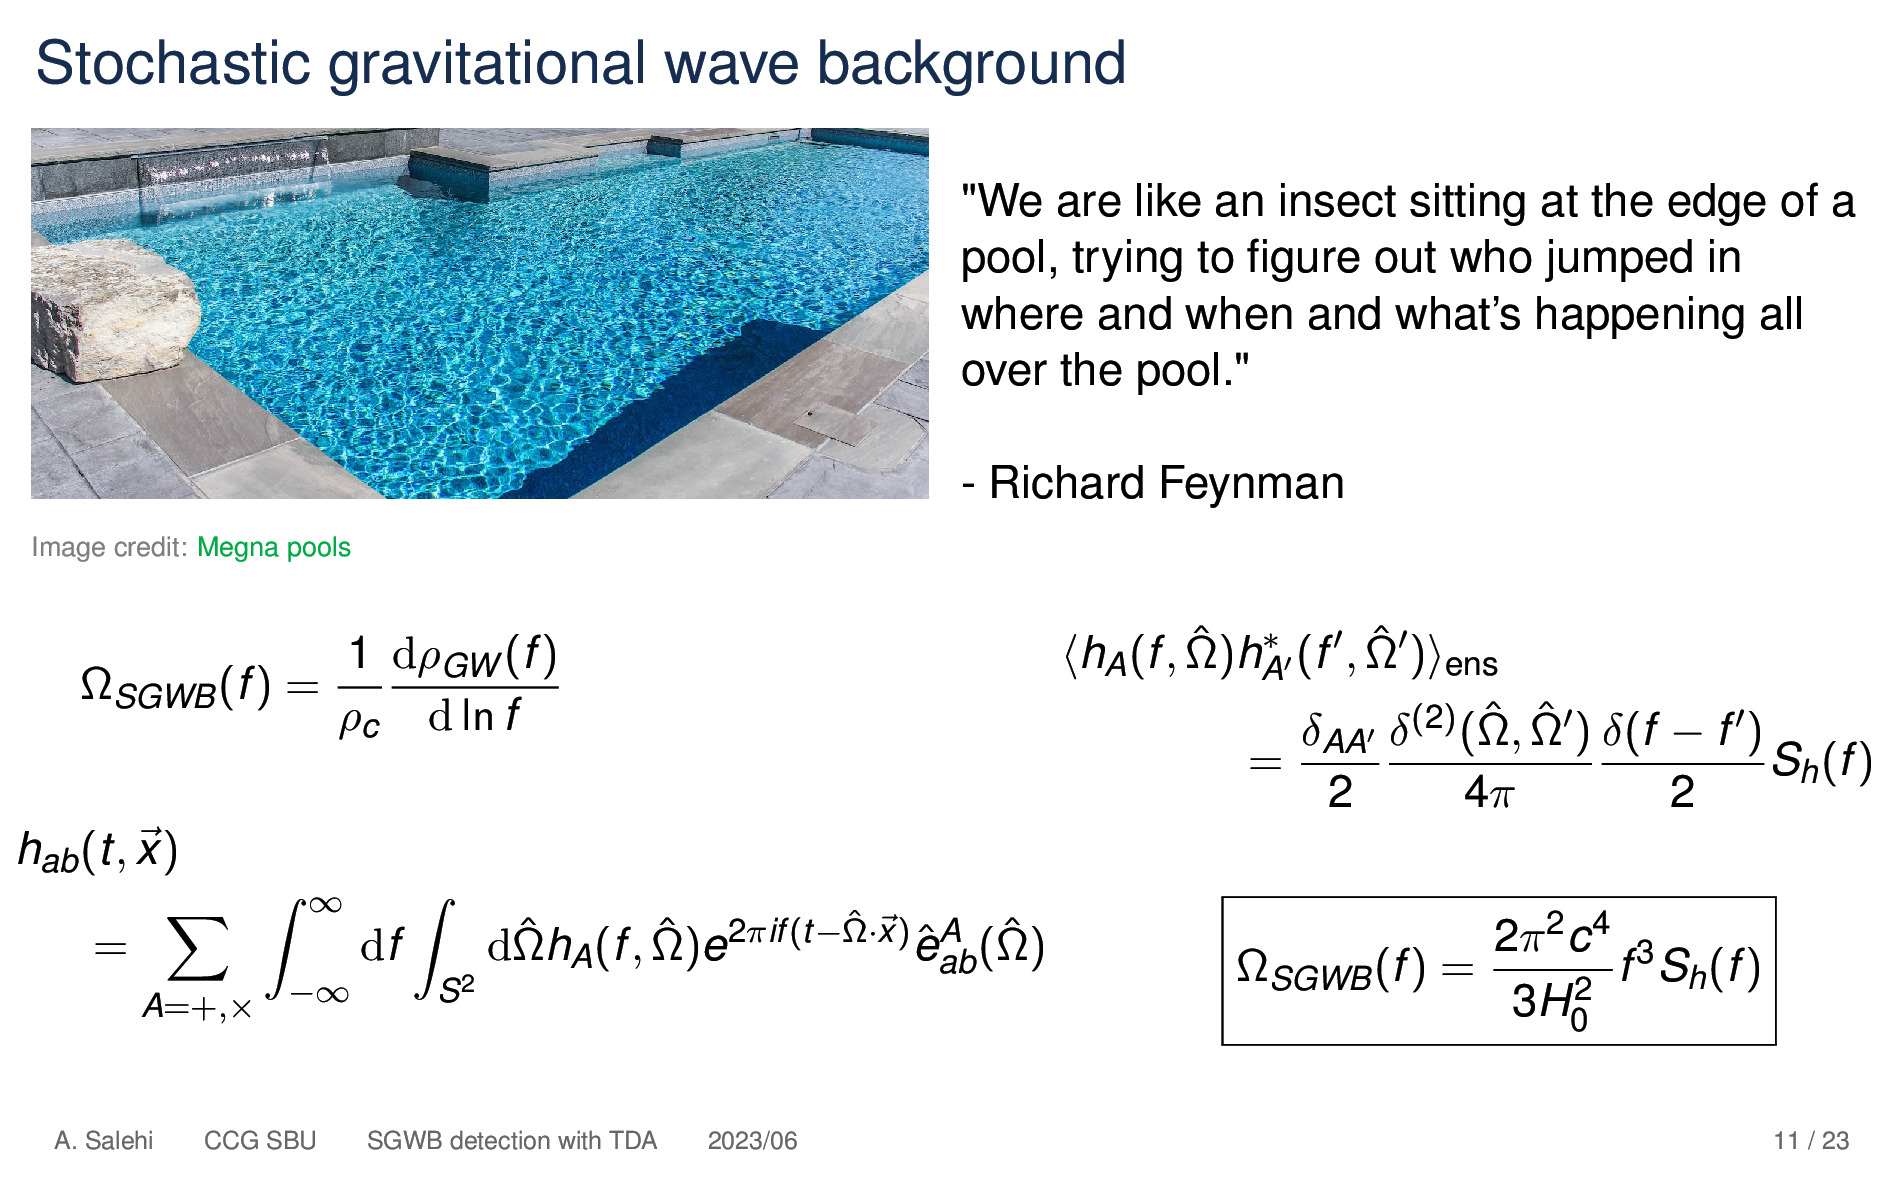
\includegraphics[width=\linewidth]{img/page-11.jpg}
			%\vspace{2ex}
			%\includegraphics[width=.95\textwidth]{img/rivus/scen-today-rivus-networks}
			%\vspace{1ex}
		\end{minipage}
	};
}
\end{tikzpicture}
\end{column}
\begin{column}{0.5\linewidth}
\begin{align*}
\uncover<+->{
	h(t) &= \int_{-\infty}^{\infty} \der f h(f) e^{2 \pi i f (t - \phi)} \\~\\
}
\uncover<+->{
	\langle h(f) h^\star (f^\prime) \rangle &= \frac{\delta (f-f^\prime)}{2} S_h(f) \\
}
\end{align*}
\uncover<+->{To achieve this we used \textit{LALSuite} package with a few added features:}
\begin{itemize}[<+->]
	\item A new data structure to read the numerical spectrum
	\item New functions to simulate SGWB for pawr-law and numerical spectra
	\item Options to access these new functionalities with an app
\end{itemize}
\end{column}
\end{columns}
\end{frame}


\begin{frame}{Spectral energy density plots (theoretical)}
\centering
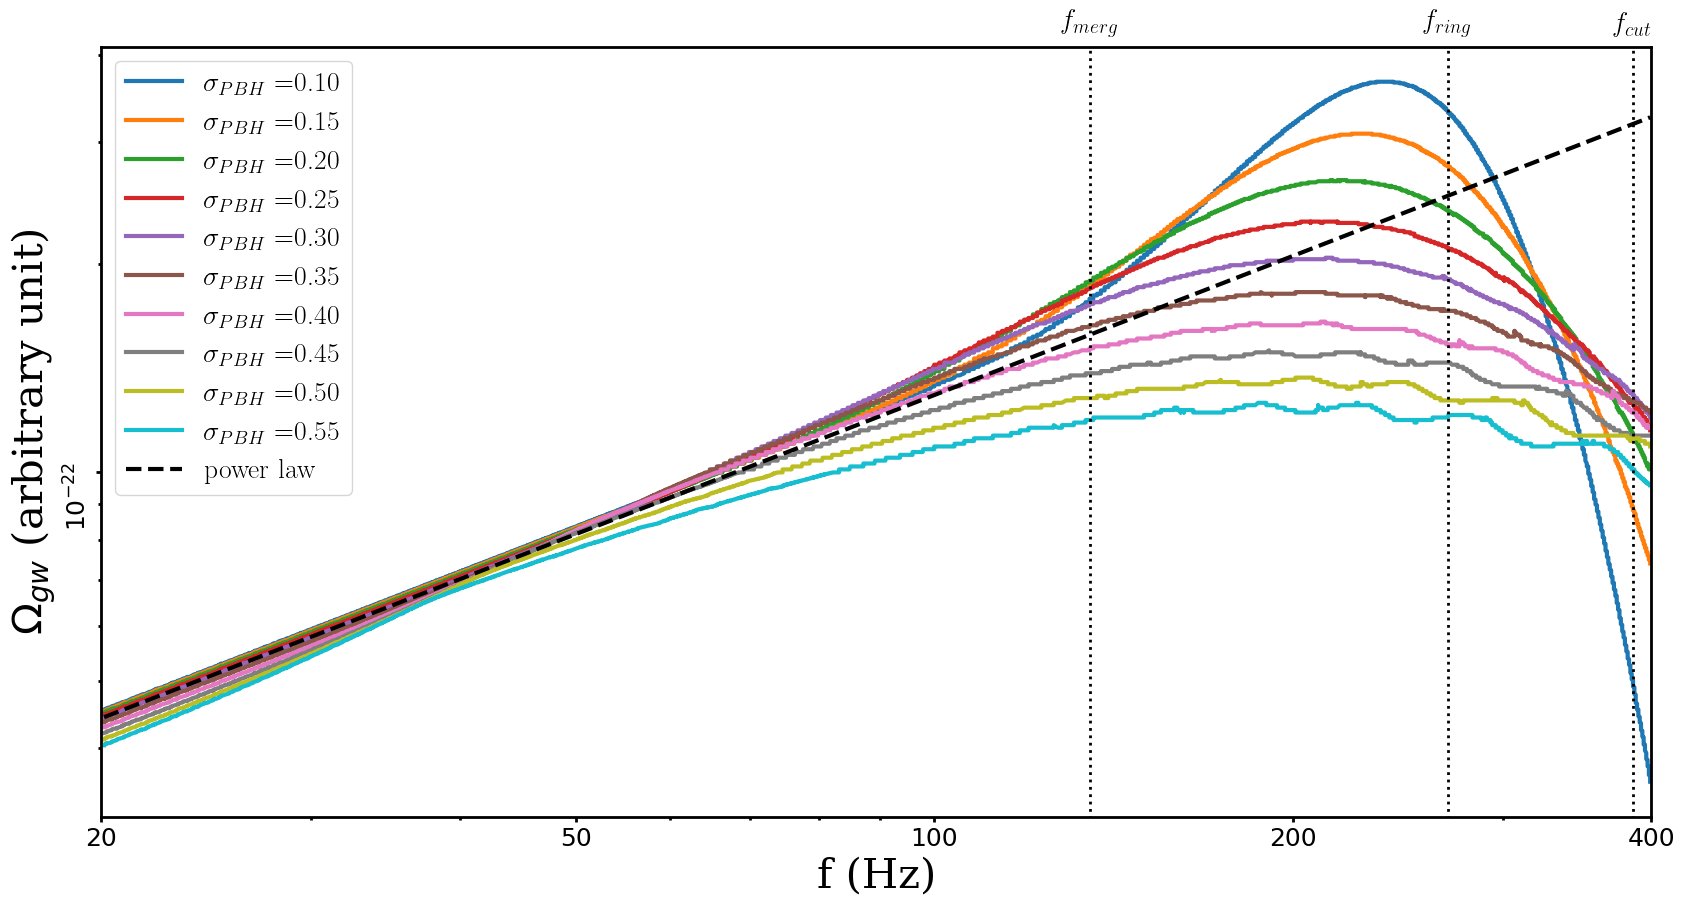
\includegraphics[width=.9\linewidth]{img/theoretical}
\end{frame}

\begin{frame}{Spectral energy density plots (numerical)}
	\centering
	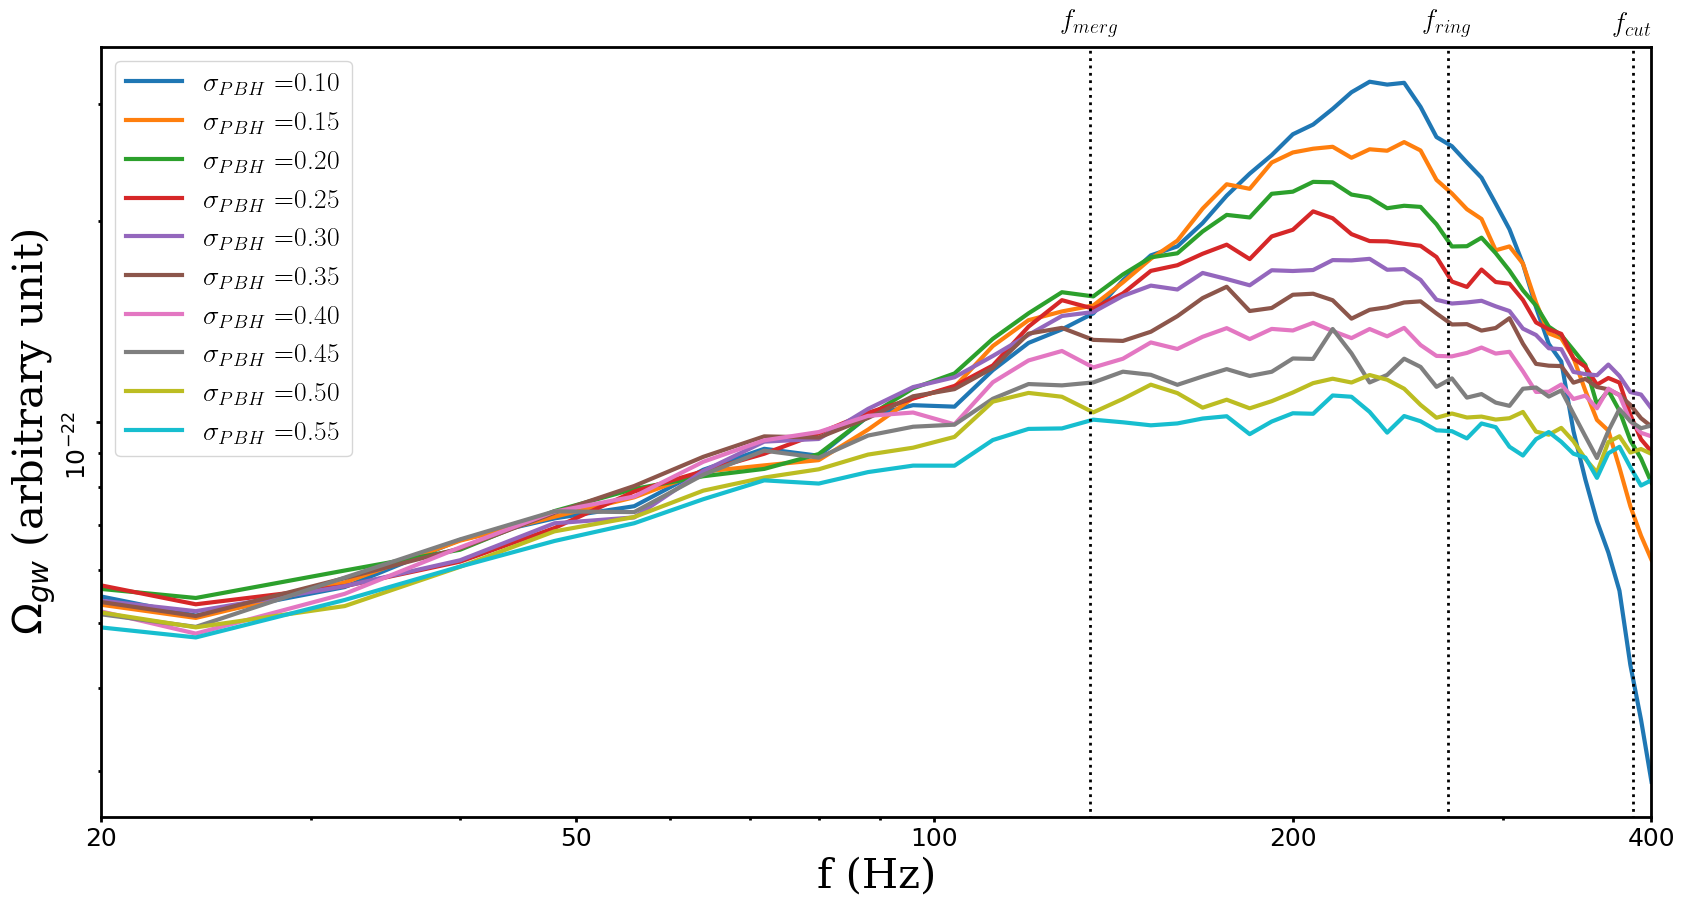
\includegraphics[width=.9\linewidth]{img/numerical}
\end{frame}

\begin{frame}{Spectral energy density plots (noisy)}
	\centering
	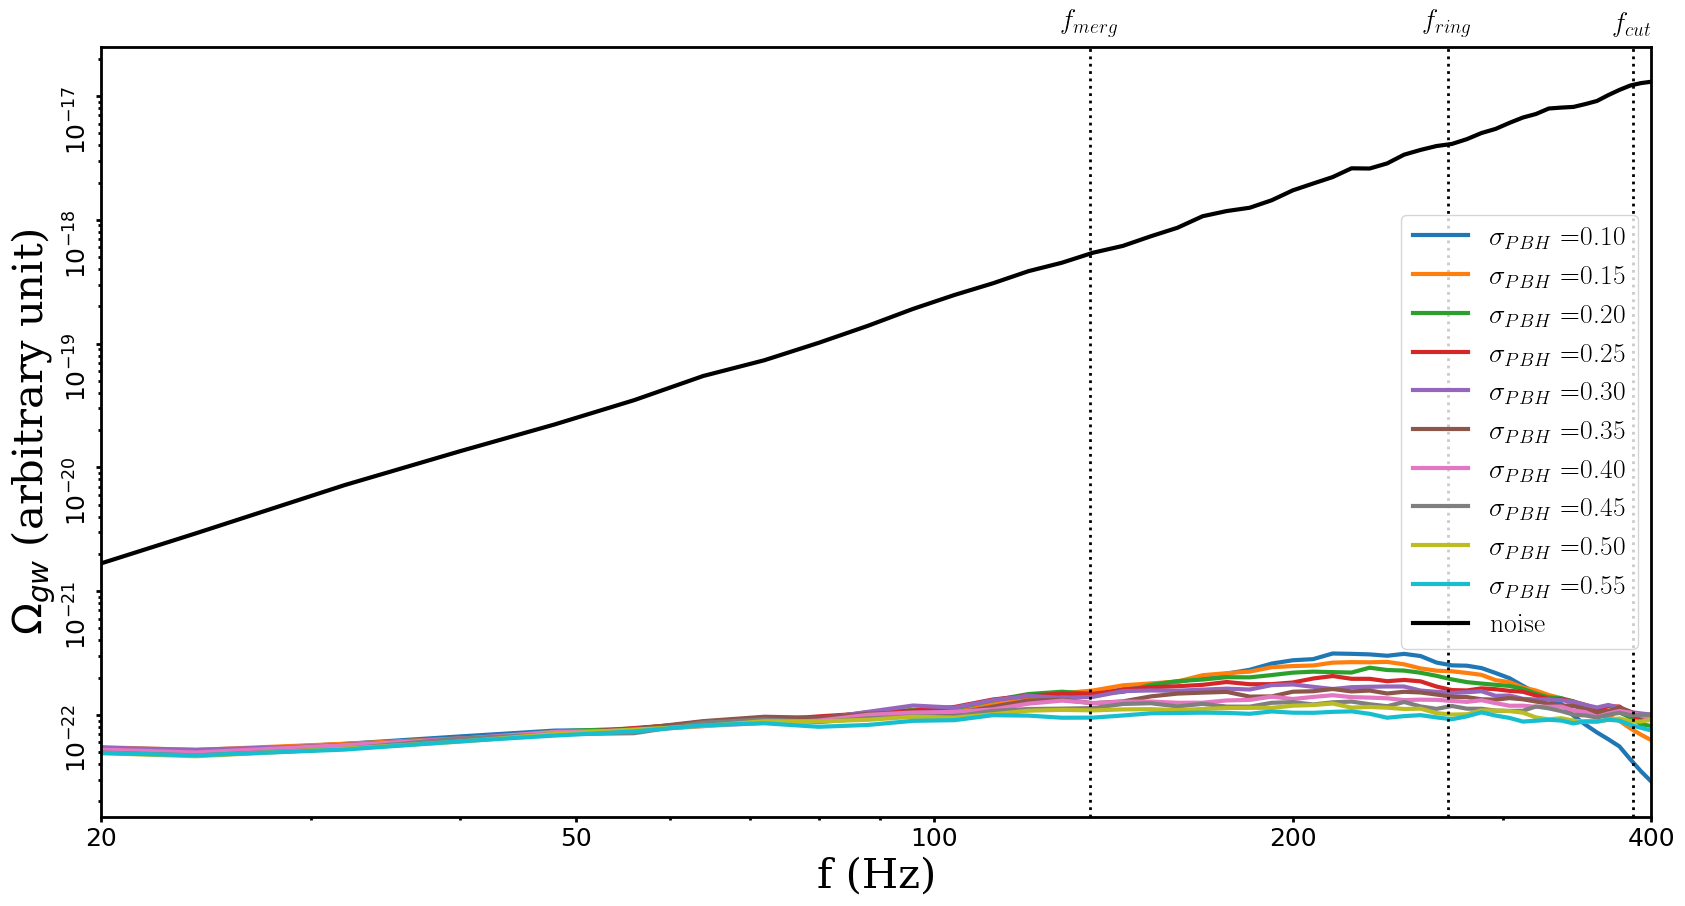
\includegraphics[width=.9\linewidth]{img/noisy}
\end{frame}

\begin{frame}{Recap}
	\uncover{We want to detect:}
	\begin{itemize}
		\item A stochastic gravitational wave background
		\item Coming from binary black hole mergers
		\item Our chosen black holes to study have a primordial origin
	\end{itemize}
	\vskip 1cm
	\uncover{To achieve these, we need:}
	\begin{enumerate}
		\item \sout{Learn about primordial black holes and their population statistics}
		\item \sout{Build a model for their merger rates based on the population statistics}
		\item \sout{Simulate a stochastic gravitational wave background}
		\item Build a model to analyse the data
		\item Run the analyses
	\end{enumerate}
\end{frame}